% Possible background additions:
% Positive/Negative examples ILASP.
% Semantic parsing maybe.

% Add a box plot somewhere


\chapter{Project Work}

This is temporary section until the project structure becomes more clear

\section{Learning to Extract Sentences}

Conditions that we wanted to achieve.

\subsection{Definitions}

There are two definitions that are used throughout the section:

% TODO add reference %
\textbf{Atomic Sentence:} A sentence is atomic if it cannot be decomposed in multiple simpler ones. Note that this equivalent to the definition used in logic.
However, the sentence structure considered in this project is often much more complex than the one considered in logics.


\textbf{Concept Sentence:} A syntactic generalisation of an atomic sentence, which satisfies the following 3 conditions:

 1. It is a valid sentence in its own right.
 
 2. True if the atomic sentence is.
 
 3. Obtained only through syntactic manipulation of an atomic sentence, a result of modifying the syntax tree of the sentence.
 
Concept sentences are often referred to as (syntactic) generalisations of a sentence in this report.



\textbf{Example number}: Splitting a given sentence into all its concepts sentences. 

Starting from the sentence: \\
\textit{The batter caught the ball in the air and sent it into the left field.} \\
we can extract the following atomic sentences: \\
\textit{The batter made contact with the ball in the air. The batter sent it into the left field.}
From these two sentences we can obtain four concept sentences: \\
\textit{The batter made contact with the ball in the air. The batter made contact with the ball. The batter sent it into the left field. The batter sent it into the field.}


The reason the project aims to extract all concept sentences from a particular sentence is two-fold:

 1. Concept sentences help associated differently worded explanations of the same concept.

 2. The final generated sentences are immediately usable for explanations.

\subsection{Problem Modelling}

% TODO: check if I am using generalisation

% INSERT reference
Inductive Logic Programming is approach is slightly different in the levels of commitment of knowledge representation than Deep Learning.
Deep Learning does not give any inductive bias to machine at all. 
The model must learn how to solve the problem from the data only.

Inductive Logic Programming uses a slightly weakened approach. 
We encode all the structure of the logic to learner which is encouraged to find all the possible theories within that structure and return the best one. 


% TODO: insert diagram for my overall pipeline.

\subsubsection{Preprocessing}

Before defining the logic structure that the learner should follow we need to learn how to encode the problem.

We are dealing with short text fragments which are first split into sentences.


% TODO: talk about the properties we would ideally like to achieve.
% Then mention usual stuff
% Then talk about ours.

Ideally we want to capture all the ways a human could explain that a particular event occurred.
In particular, we want the representation to satisfy the following:

1. Capture dependencies between words to determine whether a word is crucial to the meaning of a sentence.

2. Allow recognising slight word variations such as replacing words with its synonyms. It would be beneficial that words with same meaning are captured with a same representation.

3. Be compact. Smaller representations are quicker to process. 

4. Be domain independent. The framework itself should be translatable to different domains, so the representation should not contain domain-specific information.

5. Be interpretable. This is a requirement arising from a use of logic-based system.


% TODO: fix this section.
A common approach to encoding a word involves using concatenated dense-vector contextualised emdeddings of words. 
% INSERT references
Transformers, such as BERT, improve upon these embeddings by using self-attention mechanism to provide an even better representation for a sentence.
Dense-vector embeddings are useful because they are compact and tend to capture semantics of words (i.e. map similar words to similar value embeddings).

However, they are not interpretable making them unusable with our problem. 
But, our learning approach follows a similar idea of trying to capture the semantic relationships within a sentence.
We use dependency parse tree as a basis for both of our inductive logic learning tasks as it captures syntactic relationships between words.
Note that these are approximations of the semantic relationships between words.
In addition, words themselves are into the logical predicates.

Dependency tree gives rise to the following predicate:
\begin{verbatim}
    dep(l, token1, token2).
\end{verbatim}

It represents that there exists an arc from \textit{token1} to \textit{token2} with label \textit{l}.

Furthermore, it was noticed that in the examples for both concept and atomic sentence learning contained only the words used in the starting sentence.

As such, the problem which we are tacking could be modelled as whether or not we want to include the word in atomic/concept sentence.
These are denoted with predicates:
\begin{verbatim}
   in_generalised_sent(T). in_atomic_sent(T). 
\end{verbatim}
which represent that a token T is included in concept/atomic sentence given.

The possibility of multiple sentences arising from a given one is modelled with multiple answer sets. 



Unfortunately, this approach does not allow capturing slight word variations.
% TODO: write in which section it is described
However, these are handled at grouping stage which use the transfomer-based embeddings which have the necessary property. \\




% Consider making this as a diagram if it is too long.
\textbf{Example:} Converting a \emph{He threw a fast ball.} to a logical form and back.


1. Construct the dependency tree for a given sentence. For \emph{He threw a fast ball.} the dependency graph is shown at \ref{example-dependency-graph}.

2. Convert tokens in the tree to a logical form:

\begin{verbatim}
    token(tok0, "he").
    token(tok1, "threw").
    token(tok2, "a").
    token(tok3, "fast").
    token(tok4, "ball").
    token(tok5, ".").
\end{verbatim}

3. Convert arcs and root in a tree to predicates.
\begin{verbatim}
    root(tok1).
    dep(nsubj, tok1, tok0).
    dep(dobj, tok1, tok4).
    dep(punct, tok1, tok5).
    dep(det, tok4, tok2).
    dep(amod, tok4, tok3).
\end{verbatim}


\begin{figure}[h]
\caption{Dependency graph of \emph{He threw a fast ball.}}
\centering
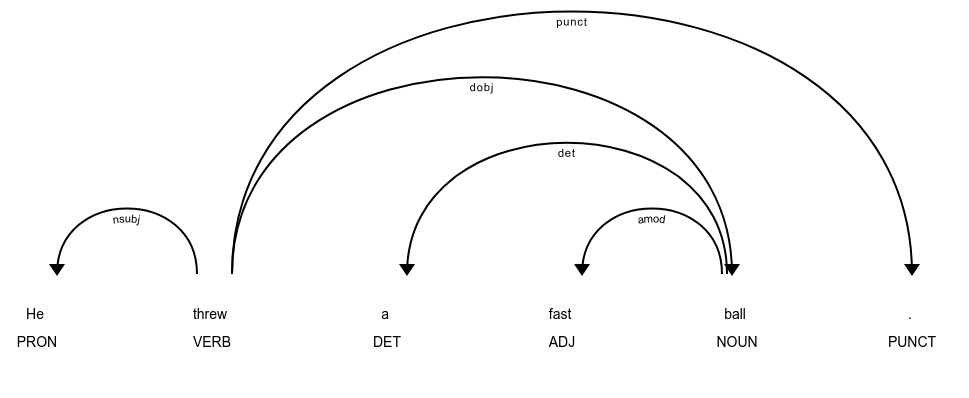
\includegraphics[width=\textwidth]{project-work/example_dependency_tree.png}
\label{example-dependency-graph}
\end{figure}

3. \textit{Clingo} is applied with atoms and predicates existing in: the background file, the learned solution file, and the generated logical form.

The resulting output is similar to:
\begin{verbatim}
Answer set #1:
{in_generalised_sent(tok0), in_generalised_sent(tok1), 
 in_generalised_sent(tok2), in_generalised_sent(tok3), 
 in_generalised_sent(tok4), in_generalised_sent(tok5)}.
    
Answer set #2:
{in_generalised_sent(tok0), in_generalised_sent(tok1), 
 in_generalised_sent(tok2), in_generalised_sent(tok4), 
 in_generalised_sent(tok5)}.
\end{verbatim}

4. For each answer set generated we reconstruct a sentence. 
The sentence reconstruction by converting each \textit{in\_generalised\_sent} token to the back to its string representation.
They are then joined by with spaces in the same order they originally appeared in.

For instance, for answer set \#2 we have tok0 -> "he", tok1 -> "threw", tok2-> "a", tok4 -> "ball", tok5 -> ".".
They are joined to a sentence \textit{he threw a ball .}

% TODO: reference truecasing
5. Post-processing clean-up involving truecasing and eliminating redundant spaces results in \emph{He threw a fast ball.} and \emph{He threw a ball.} \\



\subsubsection{Differences between atomisation and generalisation}

As noted in the previous section, atomisation and generalisation are handled in quite a similar manner.
In the current subsection, we will outline the difference between the two processes and why we have two processes in the first place.

Both are following the identical process as described in the example with only difference being in the background file and the learned solution.

Atomisation and generalisation approach generating multiple answer sets differently.
Generalisation learns the rule of the form: 
\begin{verbatim}
    in_generalised_sent(T) :- ...
    0 { in_generalised_sent(T) } 1 :- ...
\end{verbatim}
The latter rule results in two answer sets one of which contains the predicate in\_generalised\_sent, while the other one doesn't.

On the other hand, the atomisation task learns the rules of the following form:
\begin{verbatim}
    in_atomic_sent(T) :- ...
    splitting_tag(C).
\end{verbatim}
To produce multiple answer sets there are following additional rules in the background knowledge:
\begin{verbatim}
    candidate_start(T) :- splitting_tag(C), dep(C, T, _).
    candidate_start(T) :- splitting_tag(C), dep(C, _, T).
    0 { in_atomic_sent(T) : candidate_start(T) } 1.
\end{verbatim}
The idea for the latter approach is to start the atomisation from the tokens which should be in disjoint answer sets.
For example, in a sentence \emph{The ball is quick and accurate}, there is a \emph{conj} tag between \emph{quick} and \emph{accurate}.
With \emph{splitting\_tag(conj)} the learning process would be started with \emph{quick} and \emph{accurate} in different answer sets.
The rules with \emph{in\_atomic\_sent} as its head attempt to complete the sentence.
In the given example they learn to include \emph{The ball is}.
So, the overall task is to produces \emph{The ball is quick} and \emph{The ball is accurate} as final solutions.


Due to the more challenging nature of atomisation, the language bias of the learning tasks additionally includes more possible body predicates such as \emph{candiate\_start} and \emph{adjacent\_subj}.
The former is true for tokens which started the split while the latter recongises whether the sentence subject adjacent to currently included tokens.


\subsection{Example Encoding}

Generalisation and atomisation examples are given in the identical format.
Both consists of a given sentence followed by 1 to many sentences which are ways in which the provided sentence can be generalised/atomised.

Ideally, we want that the solution learned by ILASP produces possible solutions equal to the number of generalisations/atomisations.
% Equivalently, the number of answer sets produced for each sentence S be equal should be equal to the number of generalisations/atomisations of S.
% TODO: refer to background
ILASP allows defining two types of examples as outlined in \textit{section X}:


 - \#pos(ILASP)/$E^+$(definition), where $\forall<e, C> \in E^+$, $\exists A \in AS(B \cup C \cup H)$ such that $A$ extends $e$.
 
 - \#neg(ILASP)/$E^-$(definition), where $\forall<e, C> \in E^-$, $\nexists A \in AS(B \cup C \cup H)$ such that $A$ extends $e$.
 
Using these two constructs it is possible to define that we want exactly answer set for each possible generalisation/atomisation.
In particular, it is done by creating a positive example for each sentence that wish to produce. 
In addition, for each sentence example, a negative example is produced with \textit{goal} predicate in the exclusion, which defined in the context of the example. That predicate is true if in\_atomic\_sent/in\_generalised\_sent atoms are exactly corresponding to a positive example. \\


\textbf{Example}: Generating an ILASP-compatible examples for generalisation.

We will be encoding a premise sentence \textit{He threw a fast ball.} which can be generalised to: \textit{He threw a fast ball.} and \textit{He threw a ball.}

% TODO: insert reference.
1. Convert the premise sentence to logical form. This was shown in example X, so will not be shown again. 

2. For each possible generalisation, create a positive example. The context consists of predicates produced in 1) while the inclusion/exclusion appropriate in\_generalised\_sent tokens. For instance, \textit{He threw a ball.} would yield a following example:
\begin{verbatim}
#pos(example_id@noise_penalty,
{in_generalised_sent(tok0), in_generalised_sent(tok1), 
 in_generalised_sent(tok2), in_generalised_sent(tok4), 
 in_generalised_sent(tok5)},
{in_generalised_sent(tok3)}, % tok3 = "fast"
{
% all the predicates generated in 1)
}).
\end{verbatim}

3. Generate a negative example as follows:
\begin{verbatim}
#neg(example_id@noise_penalty,
{ },
{ goal },
{
% all the predicates generated in 1)

% He threw a fast ball.
goal :- in_generalised_sent(tok0), in_generalised_sent(tok1), 
        in_generalised_sent(tok2), in_generalised_sent(tok3), 
        in_generalised_sent(tok4), in_generalised_sent(tok5).
% He threw a ball.
goal :- in_generalised_sent(tok0), in_generalised_sent(tok1), 
        in_generalised_sent(tok2), in_generalised_sent(tok4), 
        in_generalised_sent(tok5)}, not in_generalised_sent(tok3).
}).
\end{verbatim}


\section{Managing Scalability Constraints}

% INSERT reference for this. %
A large challenge with logic based learning systems, such as ILASP, is a lack of scalability when dealing with large scale AI problems compared to other forms of machine learning.
The particular challenge that needed to be mitigated is the lack of scalability w.r.t size of the hypothesis space, which arises due to ILASP enumerating search space $S_M$ in full before finding a solution.
For example, consider the following simplified language bias definition:
\begin{verbatim}
#modeh(in_generalised_sent(var(token))).

#modeb(in_generalised_sent(var(token))).
#modeb(root(var(token))).
#modeb(dep(const(label), var(token), var(token))).

+ all the constant definitions.
\end{verbatim}

% Might be benficial to include a table how each rule reduced the search space size.

It took over 13 hours to generate a full search space on a machine with Intel Core i7 10510U 1.80GHz / 4.90GHz processor and 16 GiB of RAM.

% INSERT fastlas reference %
FastLAS is a system designed with alleviating this particular constraint but it is only able to deal with restricted version of learning tasks available in ILASP. 
Its inability to produce a solution with multiple answer set made it inapplicable for the current problem.
% TODO: insert reference to Mark's website
As such, the scalability issue was tackled using a meta-level definitions of the hypothesis space, which allow much greater flexibility compared to simple \textit{modeb}, \textit{modeh} statements. 
They allow constraining how rules are generated using ASP syntax.

Here are some examples of they are utilsed to restrict the search space presented in this section:
\begin{verbatim}
% Idea #1: Dep represents an arc in a tree. This allows 
% cutting out rules which are impossible to be satisfied.
    
% It is impossible to have more than 1 root per example.
:- #count{T : body(root(T))} > 1.

% Trees cannot have a relation to itself.
:- body(dep(_, X, X)).
:- body(naf(dep(_, X, X))).

% Trees are not reflexive
:- body(dep(_, X, Y)), body(dep(_, Y, X)).

% No depenency can go to the root
:- body(root(X)), body(dep(_, _, X)).

% Idea #2: Only allow two dep rules to occur in a body
% under certain conditions. 

% Pairs of dependency tags which can co-occur.
% Much smaller set of all possible pairs.
dep_chain(prep, pobj).
dep_chain(pobj, amod).
...

% Allow any rule with at most one dep predicate
allowed_dep_rule :- #count{L, V4, V5 : body(dep(L, V4, V5))} <= 1.
% Allow rule with two dep predicates if it is labels are white-listed
% as approved dep_chains and tokens are chained too.
allowed_dep_rule :- body(dep(L1, _, V2)), body(dep(L2, V2, _)), 
                    dep_chain(L1, L2), 
                    #count{L, V4, V5 : body(dep(L, V4, V5))} = 2.

:- not allowed_dep_rule.
\end{verbatim}

These kinds of modifications allowed the search space generation times to take less than a minute, starting from over 13 hours.


% Talk about memory when we actually fix it.
Probably need to talk a bit about memory if it is possible.


\section{Evaluation}

\subsection{Used Metrics}

Both atomisation and generalisation problems had an set of solutions of unknown size.
As such, an ideal metric would higher score if 2 sets are very similar compared to those that are far apart.

That would ideally involve a similarity in number of produced solutions and similarity of the elements themselves.

Due to this reason, a single number would have been hard to interpret since it would make it unclear what kinds of mistakes the model is making. 
For that reason, the evaluation is done with metrics which work with sets with possibly reduced notion of element equality.

The simplest metrics used were per-example Jaccard Index, precision and recall, with exact equality.
Jaccard Index is a metric with the following form:

 - $Jaccard(A, B) = \frac{card(A \cap B)}{card(A \cup B)}$ where $card$ represents set cardinatlity, $A$ a set containing true solutions, while $B$ contains predicated solutions.\\
 
Precision and recall are equivalent to the following for the problems in this thesis:
 
  - $Precision(A, B) = \frac{number \; of \; correctly \; predicted \; sentences}{number \; of \; predicated \; sentences} = \frac{card(A \cap B)}{card(B)}$
  
  - $Recall(A, B) = \frac{number \; of \; correctly \; predicted \; sentences}{number \; of \; correct \; sentences} = \frac{card(A \cap B)}{card(A)}$ \\
where  $card$ represents set cardinatlity, $A$ a set containing true solutions, while $B$ contains predicated solutions.

These metrics are also evaluated in a slightly relaxed manner using Levensthein distance.
$Jaccard\text{-}k$ is a notation used in this report where two elements of a set are equal if their Levensthein distance is less or equal $k$.
The same notational trick is used for $Recall\text{-}k$ and $Precision\text{-}k$.


% TODO: talk about consistency across runs for ILASP with cut-off 

% TODO: limitations
% - dependency parsing not perfect


% TODO: rename precision and recall with generalisation-precision/generalistaion-recall
